\subsection{Point lights}
In the game, spotlights are represented by white spherical lamps.

In Euclidean geometry, assuming that a point light is placed at a point $p$ and that the current fragment's position is given by $f$, we can calculate the light direction vector $l$ simply as
\begin{equation*}
    l = \frac{p - f}{d_E(p, f)},
\end{equation*}
where $d_E$ is the usual Euclidean distance, i.e.
\begin{equation} \label{eq:dist-euclidean}
    d_E(a, b) = \sqrt{\langle a - b, a - b\rangle_E}.
\end{equation}
For non-Euclidean geometries, we use modified formulas given by \cite{Szirmay-Kalos2022}, namely
\begin{equation}
    l = \frac{p - f \cos(d_S(p, f))}{\sin(d_S(p, f))}
\end{equation}
for spherical geometry and
\begin{equation}
    l = \frac{p - f\cosh(d_H(p, f))}{\sinh(d_H(p, f))}
\end{equation}
for hyperbolic geometry.
The spherical and hyperbolic distances $d_S$ and $d_H$ are given by
\begin{equation} \label{eq:dist-spherical}
    d_S(a, b) = \cos^{-1}(|\langle a, b \rangle_E|)
\end{equation}
and
\begin{equation} \label{eq:dist-hyperbolic}
    d_H(a, b) = \cosh^{-1}(-\langle a, b \rangle_L)
\end{equation}
respectively.

The important difference between a point light and a directional light is the \textit{attenuation} $a$.
Attenuation represents how the light's strength diminishes over distance.
It can be expressed as a reciprocal of a quadratic function:
\begin{equation}
    a = \frac{1}{K_c + K_l d + K_q d^2},
\end{equation}
where $d$ is the distance of the fragment from the source that can be calculated using one of the formulas \ref{eq:dist-euclidean}, \ref{eq:dist-spherical}, or \ref{eq:dist-hyperbolic} depending on the geometry.
Multiplying the light by the attenuation factor gives the desired effect of a realistic point light source such as a lamp, see \autoref{fig:point-lights}.
\begin{figure}[h]
    \centering
    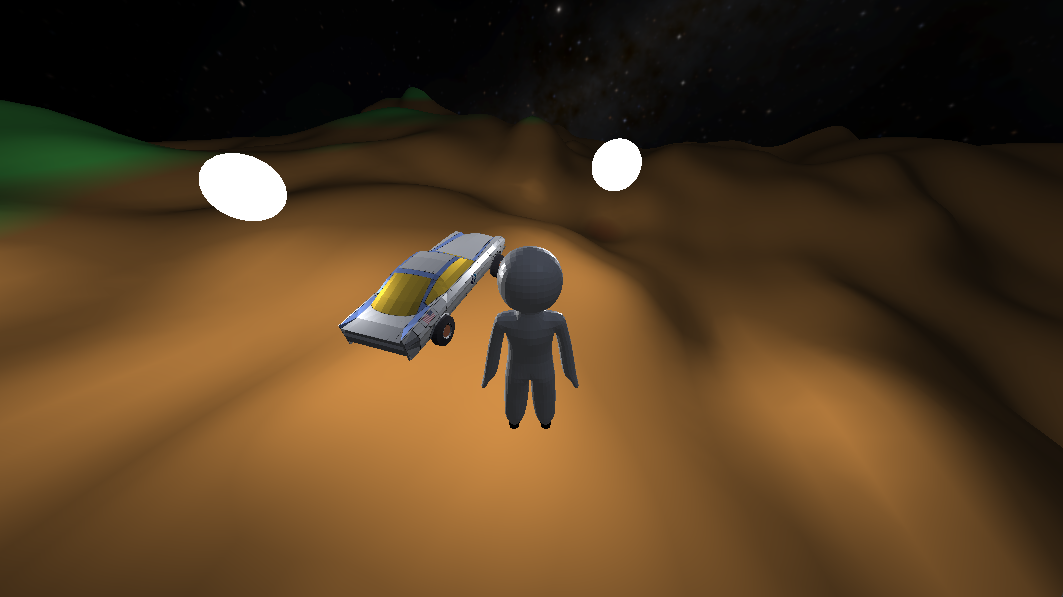
\includegraphics[width=0.8\textwidth]{chapters/lighting/sections/lighting/resources/point-lights.png}
    \caption{Point lights}
    \label{fig:point-lights}
\end{figure}
Point lights in hyperbolic and spherical geometry are shown in \autoref{fig:point-light-non-euc}.
\begin{figure*}[h]
    \centering
    \begin{subfigure}[b]{0.475\textwidth}
        \centering
        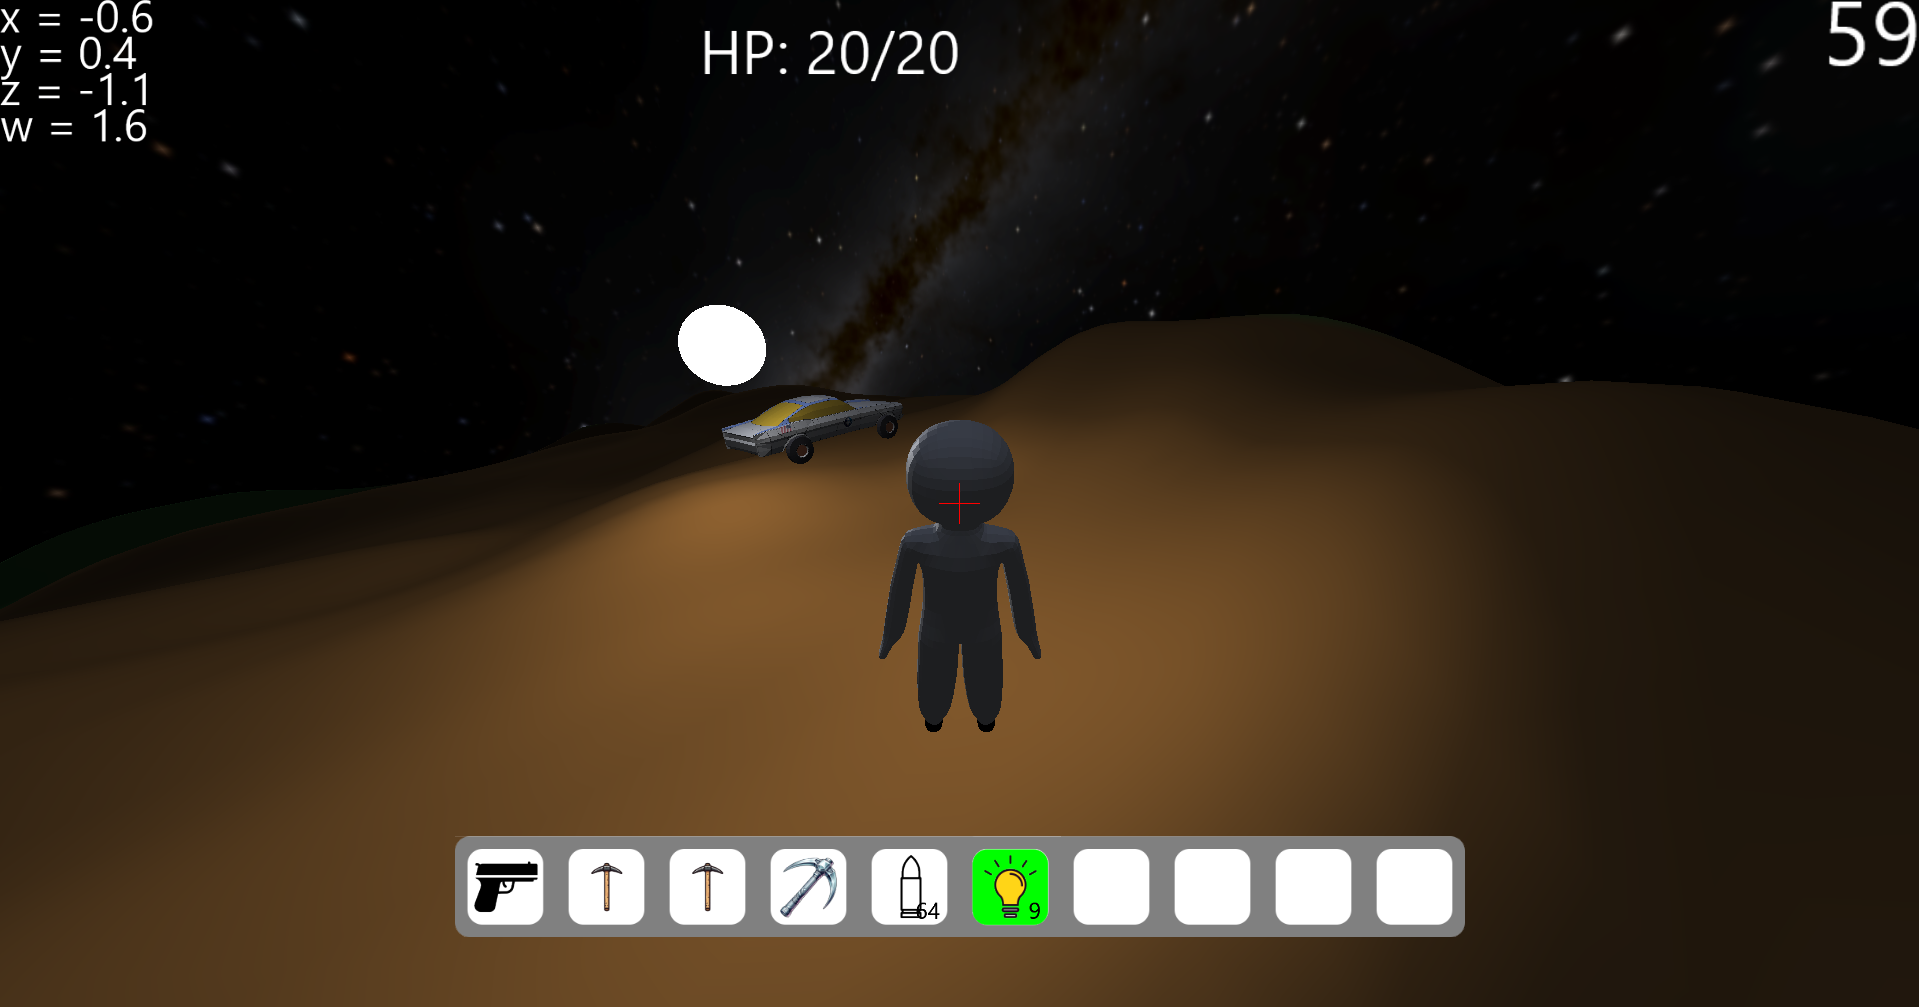
\includegraphics[width=\textwidth]{chapters/lighting/sections/lighting/resources/point-light-hyperbolic.png}
        \caption[]%
        {{\small Hyperbolic space}}
        \label{fig:point-light-hyperbolic}
    \end{subfigure}
    \hfill
    \begin{subfigure}[b]{0.475\textwidth}
        \centering
        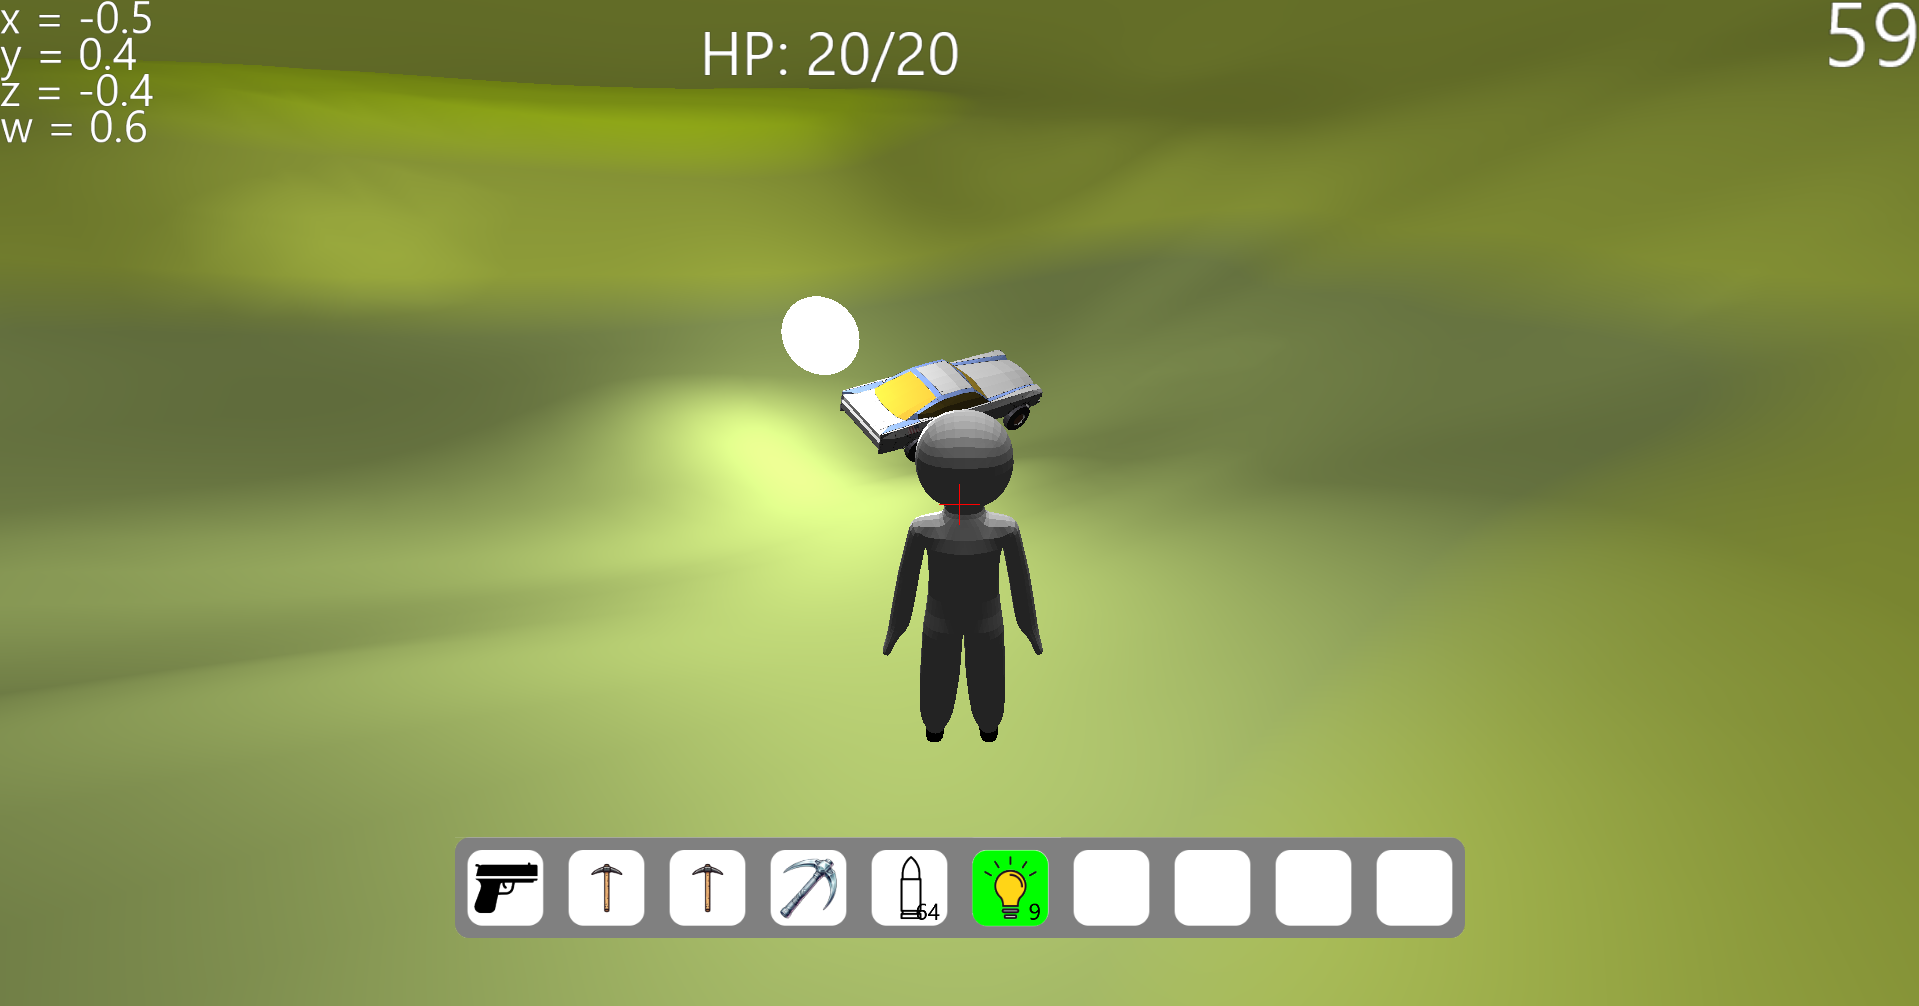
\includegraphics[width=\textwidth]{chapters/lighting/sections/lighting/resources/point-light-spherical.png}
        \caption[]%
        {{\small Spherical space}}
        \label{fig:point-light-spherical}
    \end{subfigure}
    \caption[]
    {\small Point lights in non-Euclidean spaces}
    \label{fig:point-light-non-euc}
\end{figure*}